\documentclass[a4paper,11.5pt]{article} % тип документа


%%%Библиотеки
%\usepackage[warn]{mathtext}
\usepackage[T2A]{fontenc} % кодировка
\usepackage[utf8]{inputenc} % кодировка исходного текста
\usepackage[english,russian]{babel} % локализация и переносы
\usepackage{caption}
\usepackage{listings}
\usepackage{amsmath,amsfonts,amssymb,amsthm,mathtools}
\usepackage{wasysym}
\usepackage{graphicx}%Вставка картинок правильная
\usepackage{float}%"Плавающие" картинки
\usepackage{wrapfig}%Обтекание фигур (таблиц, картинок и прочего)
\usepackage{fancyhdr} %загрузим пакет
\usepackage{lscape}
\usepackage{xcolor}
\usepackage[normalem]{ulem}
\usepackage{hyperref}

%%%Конец библиотек




%%%Настройка ссылок
\hypersetup
{
colorlinks=true,
linkcolor=blue,
filecolor=magenta,
urlcolor=blue
}
%%%Конец настройки ссылок


%%%Настройка колонтитулы
\pagestyle{fancy}
\fancyhead{}
\fancyhead[L]{Лаб. работа 2.5.1}
\fancyhead[R]{Талашкевич Даниил, группа Б01-009}
\fancyfoot[C]{\thepage}
%%%конец настройки колонтитулы



\begin{document}
%%%%Начало документа%%%%


%%%Начало титульника
\begin{titlepage}

\newpage
\begin{center}
\normalsize Московский физико-технический институт \\(госудраственный университет)
\end{center}

\vspace{6em}

\begin{center}
\Large Лабораторная работа по термодинамике\\
\end{center}

\vspace{1em}

\begin{center}
\large \textbf{Измерение коэффициента поверхностного натяжения жидкости [2.5.1]}
\end{center}

\vspace{2em}

\begin{center}
\large Талашкевич Даниил Александрович\\
Группа Б01-009
\end{center}

\vspace{\fill}

\begin{center}
Долгопрудный \\22.02.2021
\end{center}

\end{titlepage}
%%%Конец Титульника



%%%Настройка оглавления и нумерации страниц
\thispagestyle{empty}
\newpage
\tableofcontents
\newpage
\setcounter{page}{1}
%%%Настройка оглавления и нумерации страниц


%%%%%%Начало работы с текстом%%%%%%

\section{Аннотация}
\textbf{Цель работы:} 1) измерение температурной зависимости коэффициента поверхностного натяжения дистиллированной воды с использованием известного коэффициента поверхностного натяжения спирта; 2) определение полной поверхностной энергии и теплоты, необходимой для изотермического образования единицы поверхности жидкости при различной температуре.

\textbf{В работе используются:} прибор Ребиндера с термостатом и микроманометром; исследуемые жидкости; стаканы.

\section{Теоретические сведения}

Поверхностное натяжение имеет двойной физический смысл -- энергетический (термодинамический) и силовой (механический). Энергетическое (термодинамическое) определение: поверхностное натяжение -- это удельная работа увеличения поверхности при её растяжении при условии постоянства температуры. Силовое (механическое) определение: поверхностное натяжение -- это сила, действующая на единицу длины линии, которая ограничивает поверхность жидкости

Наличие поверхностного слоя приводит к различию давлений по разные стороны от искривленной границы раздела двух сред. Для сферического пузырька с воздухом внутри жидкости избыточное давление даётся формулой Лапласа:

\begin{equation}
\Delta P = P_{inside} - P_{outside} = \frac{2\sigma}{r},
\label{eq:1}
\end{equation}

где $\sigma$ – коэффициент поверхностного натяжения, $P_{inside}$ и $P_{outside}$ – давление внутри пузырька и снаружи, $r$ – радиус кривизны поверхности раздела двух фаз. Эта формула лежит в основе предлагаемого метода определения коэффициента поверхностного натяжения жидкости. Измеряется давление $\Delta P$, необходимое для выталкивания в жидкость пузырька воздуха.

\section{Экспериментальная установка}

Исследуемая жидкость (дистиллированная вода) наливается в сосуд (колбу) $B$. Тестовая жидкость (этиловый спирт) наливается в сосуд $E$. При измерениях колбы герметично закрываются пробками. Через одну из двух пробок проходит полая металлическая игла $C$. Этой пробкой закрывается сосуд, в котором проводятся измерения. Верхний конец иглы открыт в атмосферу, а нижний погружен в жидкость. Другой сосуд герметично закрывается второй пробкой. При создании достаточного разряжения воздуха в колбе с иглой пузырьки воздуха начинают пробулькивать через жидкость. Поверхностное натяжение можно определить по величине разряжения $\Delta P$ (\ref{eq:1}), необходимого для прохождения пузырьков (при известном радиусе иглы).

\bigskip

Разряжение в системе создается с помощью аспиратора $A$. Кран К$_2$ разделяет две полости аспиратора. Верхняя полость при закрытом кране К$_2$ заполняется водой. Затем кран К$_2$ открывают и заполняют водой нижнюю полость аспиратора. Разряжение воздуха создается в нижней полости при открывании крана К$_1$, когда вода вытекает из неё по каплям. В колбах $B$ и $C$, соединённых трубками с нижней полостью аспиратора, создается такое же пониженное давление. Разность давлений в полостях с разряженным воздухом и атмосферой измеряется спиртовым микроманометром (устройство микроманометра описано в Приложении).
Для стабилизации температуры исследуемой жидкости через рубашку $D$ колбы $B$ непрерывно прогоняется вода из термостата.

%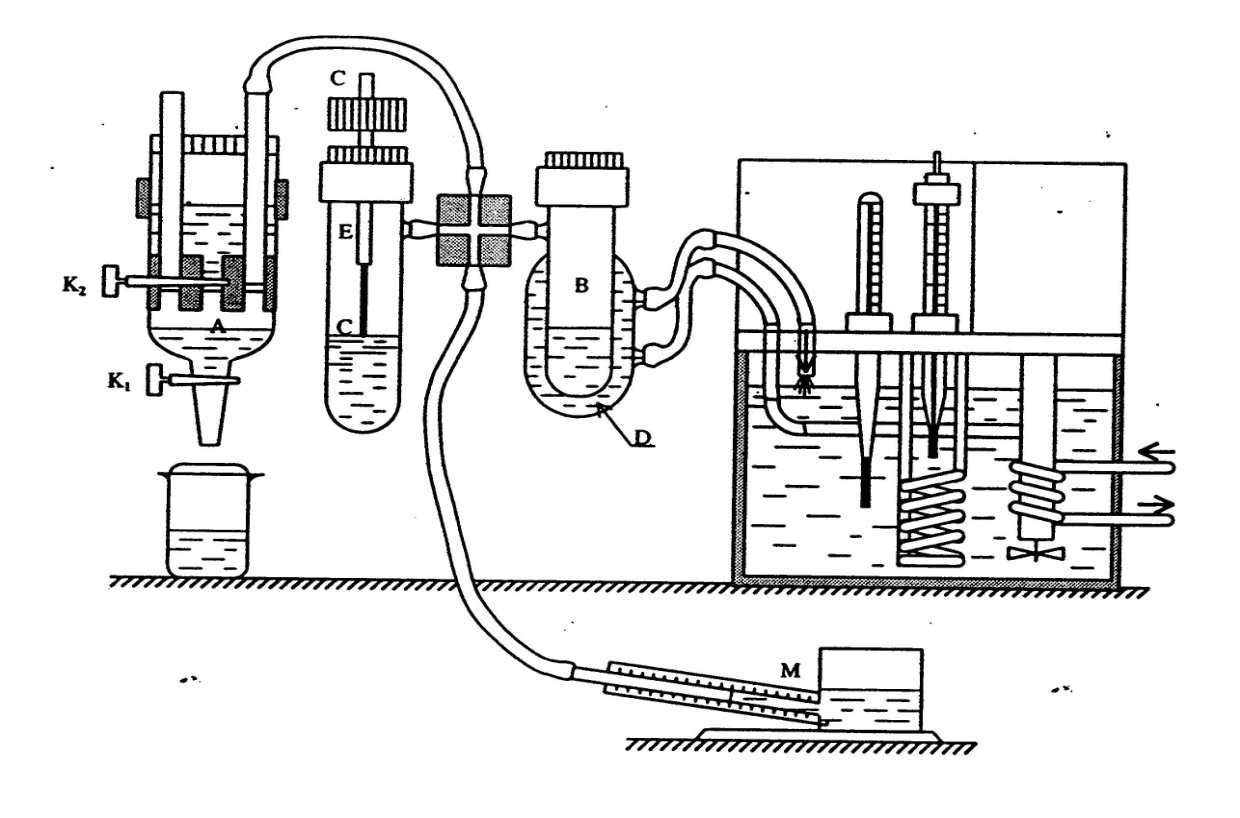
\includegraphics[width=1\textwidth]{Scheme.jpg}

Обычно кончик иглы лишь касается поверхности жидкости, чтобы исключить влияние гидростатического давления столба жидкости. Однако при измерении температурной зависимости коэффициента поверхностного натяжения возникает ряд сложностей. Во-первых, большая теплопроводность металлической трубки приводит к тому, что температура на конце трубки заметно ниже, чем в глубине жидкости. Во-вторых, тепловое расширение поднимает уровень жидкости при увеличении температуры.
Обе погрешности можно устранить, погрузив кончик трубки до самого дна. Полное давление, измеренное при этом микроманометром, $P = \Delta P + \rho gh$. Заметим, что $\rho gh$ от температуры практически не зависит, так как подъём уровня жидкости компенсируется уменьшением её плотности (произведение $\rho h$ определяется массой всей жидкости и поэтому постоянно). Величину $\rho gh$ следует измерить двумя способами. Во-первых, замерить величину $P1 = \Delta P'$, когда кончик трубки только касается поверхности жидкости. Затем при этой же температуре опустить иглу до дна и замерить $P_2 = \rho gh + \Delta P"$ ($\Delta P' ,\: \Delta P"$ – давление Лапласа). Из-за несжимаемости жидкости можно положить $\Delta P' = \Delta P"$ и тогда $\rho gh = P_2 -P_1$. Во-вторых, при измерениях $Р_1$ и $Р_2$ замерить линейкой глубину погружения иглы $h$. Это можно сделать, замеряя расстояние между верхним концом иглы и любой неподвижной частью прибора при положении иглы на поверхности и в глубине колбы.

\section{Измерения}

Проведем измерения для спирта. Для этого установим частоту падения капель из аспиратора около 1 капли в 5 секунд. Измерим максимальное добавочно давление в системе. Полученный результат $\Delta p = 40 \Rightarrow \Delta P = 78$($p$ -- единица длины на микробарометре, а $P$ уже искомое давление).

\bigskip

Далее вынем иглу, просушим ее и измерим микроскопом ее диаметр (внутренний):

\begin{equation}
d = 1.2 \pm 0.05 \text{ мм}.
\label{eq:2}
\end{equation}

Как можно увидить экспериментальный результат совпал с прямым измерение, что говорит об применимости нашей модели. Из табличного значения коэффициента поверхностного натяжения спирта $\sigma = 22.3 \text{ мн/м}$, теперь по формуле (\ref{eq:1}) получим:

\begin{equation*}
r = \frac{2\sigma}{\Delta P} = 0,6 \text{ мм}.
\end{equation*}

Как можно увидить экспериментальный результат совпал с прямым измерение, что говорит об применимости нашей модели.

\bigskip

Затем установим иглу в воду так, чтобы она едва касалась воды. Проведя измерения давления и занеся результаты в таблицу ниже получим значение $\Delta P = 6 \text{ Па}$, затем опустим иглу до дна, предварительно измерив высоту. Вновь измерим высоту:

\begin{equation}
h_1 =20 \pm 0.5 \text{ мм; } \\ h_2 =6 \pm 0.5 \text{ мм}\\ \Rightarrow \Delta h = 14 \pm 0.5 \text{ мм.}
\label{eq:4}
\end{equation}

\begin{center}
	\begin{tabular}{|c|c|c|}
	\hline 
	№ & $p_1, \text{ отн. длины}$ & $p_2 \text{ отн. длины}$ \\ 
	\hline 
	1 & 126 & 159 \\ 
	\hline 
	2 & 125 & 159 \\ 
	\hline 
	3 & 124 & 159 \\ 
	\hline 
	4 & 125 & 159 \\ 
	\hline 
	5 & 125 & 159 \\ 
	\hline
	<p>, отн. длины & 125 & 159 \\ 
	\hline
	<P>, Па & 245 & 311 \\ 
	\hline 
	\end{tabular} 
\end{center}

\bigskip

Проведем серию измерений $P_2$ для различных температур воды в интервале [20--60 $^\circ C$] (шаг $5^\circ C$), регулируемых термостатом, занесем результаты в таблице ниже.

\begin{center}
\begin{tabular}{|c|c|c|c|c|c|c|c|}
\hline
	№ & $p_2(25)$ & $p_2(30)$ & $p_2(35)$ & $p_2(40)$ & $p_2(45)$ & $p_2(50)$ & $p_2(55)$ 	\\
	\hline
	$1$ & 158 & 158 & 156 & 155 & 154 & 153 & 151 \\
	\hline
	$2$ & 158 & 157 & 156 & 155 & 154 & 152 & 152 \\
	\hline
	$3$ & 158 & 157 & 156 & 156 & 153 & 152 & 152 \\
	\hline
	$4$ & 159 & 157 & 156 & 155 & 153 & 153 & 152 \\
	\hline
	$5$ & 158 & 157 & 155 & 154 & 154 & 153 & 151 \\
	\hline
	$<p_2>$ & 158 & 157 & 156 & 155 & 154 & 153 & 152 \\
	\hline
	$<P_2>, \text{ Па}$ & 309,68 & 307,72 & 305,76 & 303,80 & 300,86 & 298,90 & 296,94 \\
	\hline
\end{tabular}
\end{center}

По полученным данные можем получить зависимость $P_2(t)$, так как мы знаем как получить давление в Па через относительную длину (показания микроманометра)

\begin{center}
\begin{tabular}{|c|c|c|}
	\hline
	$\text{t, }^\circ C$ & $P_2, \text{Па}$ & $p_2 \text{, отн. длины}$ \\
	\hline
	25 & 309,68 & 158 \\
	\hline
	30 & 307,72 & 157 \\
	\hline
	35 & 305,76 & 156 \\
	\hline
	40 & 303,80 & 155 \\
	\hline
	45 & 300,86 & 154 \\
	\hline
	50 & 298,90 & 153 \\
	\hline
	55 & 296,94 & 152 \\
	\hline
\end{tabular}
\end{center}

Такое округление обусловлено тем, что погрешность микроманометра 1 [отн. длина], а $P_i$ считает по формуле, с точностью констант до 2 знаков после запятой.

\bigskip

\section{Обработка данных}

\smallskip

Проведем пересчет экспериментальных данных для нахождения $\sigma(T)$, оценим погрешности.

\smallskip

Построим график зависимости $\sigma(T)$

\smallskip

Из график \textit{методом наименьших квадратов} найдем:

\smallskip

\begin{equation}
\frac{d\sigma}{dT} = (-0.126 \pm 0.01)\ \text{мН} \cdot \text{м} / C
\end{equation}

Сравним с табличным:

\begin{equation}
\frac{d\sigma_t}{dT} = -0.17\ \text{мН} \cdot \text{м} / C
\end{equation}

\bigskip

\section{Графики}

По полученным данным построим график $P_2(t)$:

\begin{figure}[h]
	\center{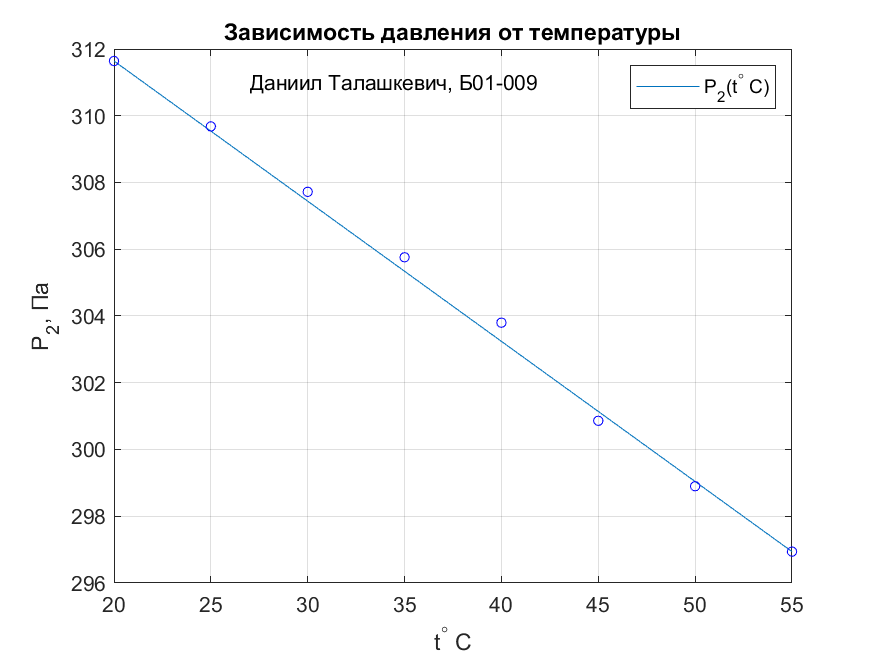
\includegraphics[scale = 0.65]{graph1.png}}
	%\caption{Сферическая система координат наглядно}
	\label{gr:1}
\end{figure}

Используя формулу (\ref{eq:1}) и по полученному $r$ капилляра построим график $\sigma(t)$:

\newpage

\begin{figure}[h]
	\center{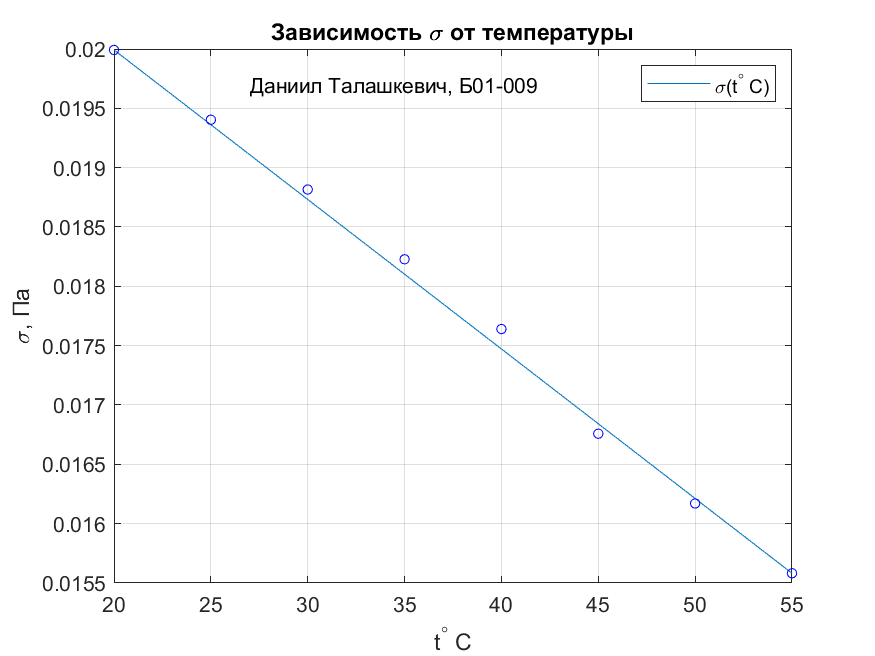
\includegraphics[scale = 0.65]{graph2.png}}
	%\caption{Сферическая система координат наглядно}
	\label{gr:2}
\end{figure}

По МНК рассчитаем коэффициент наклона, то есть $q = - T\frac{d \sigma}{d T},$ где $\frac{d \sigma}{d T} = -0,000126$. Тогда построим график $q (T)$:

\begin{figure}[h]
	\center{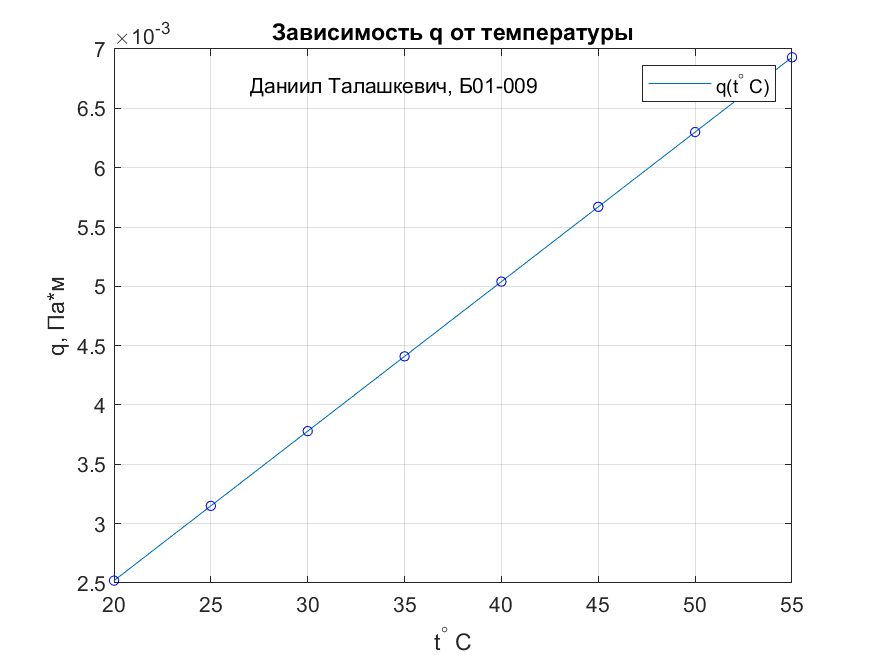
\includegraphics[scale = 0.65]{graph3.png}}
	%\caption{Сферическая система координат наглядно}
	\label{gr:3}
\end{figure}

Теперь построим график зависимости $U_\text{п}/F\ (t^\circ C)$. $U_\text{п}/F = \sigma - T\frac{d \sigma}{d T} = \sigma + q$:
\newpage
\begin{figure}[h]
	\center{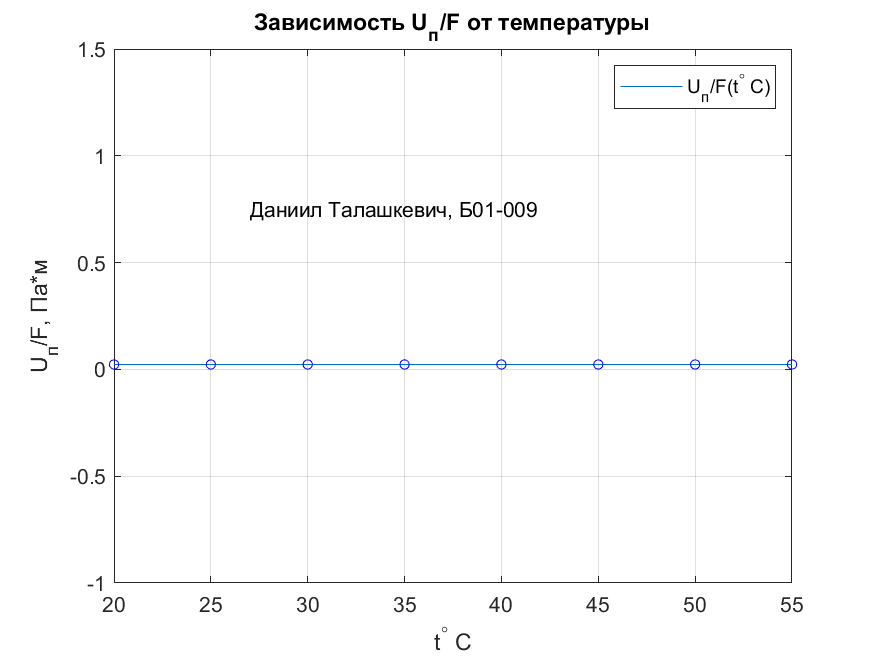
\includegraphics[scale = 0.65]{graph4.png}}
	%\caption{Сферическая система координат наглядно}
	\label{gr:3}
\end{figure}



\section{Вывод}

Теория точно описывает вид наблюдаемых зависимостей, хоть численно и отличается на величину, значительно превышающую оцененную погрешность измерений, что указывает на низкую точность представленного метода измерений, которая может быть связана с неоюходимостью учета сложных не квазистационарных процессах, происходящих при пробулькивании пузырька через жидкость.


\end{document}